\section{Molekulardynamik}
\label{md}

Ursprünglich mit dem Ziel der klassischen Simulation idealer Gase entwickelt, wurde die Molekulardynamik seither um die Fähigkeit zur Simulation von Festkörpern, organischen Molekülen und Reaktionen erweitert.
Dadurch findet sie Anwendung in Simulationen von Materialien und chemischen Stoffen bei beliebigen Temperaturen und Drücken, um deren Verhalten vorhersagen und auf reale Prozesse zurückführen zu können.

Nachfolgend möchte ich einen kurzen Überblick über die Formulierung molekulardynamischer Methoden geben (Abschnitt \ref{mdformulation}) und im Anschluss auf die Unterschiede und Möglichkeiten der Kraftfelder eingehen (Abschnitt \ref{mdforcefields}).

\subsection{Formulierung}
\label{mdformulation}

Molekulardynamik ist eine klassische Vielteilchenmethode, die jedem Teilchen des Systemes \todo{wieso $R$?}$R$ eine Masse $m$, eine Position $\vec r$, einen Impuls $\vec p$ und Kräfte entsprechend eines lokalen Kraftfeldes $\vec{F}(R)$ oder eventuellen Randbedingungen zuweist.
Entsprechend der Born-Oppenheimer-Näherung, nach der die Elektronen eines chemischen Systemes an ihre Atomkerne gebunden sind und schnell genug auf Änderungen des Systemes reagieren, genügt es, die Atome als Punktmassen an der Position ihres Atomkernes zu betrachten.
Elektronische und sonstige Interaktionen werden dann durch die verwendeten Kraftfelder beschrieben, die ihrerseits Annäherungen vornehmen können, um die Simulationszeit auf Kosten der Genauigkeit zu verringern.

Der Systemzustand wird dann entweder entsprechend des gewählten Ensembles zeitlich integriert, oder hinsichtlich der Energie des Gesamt- oder eines Teilsystemes optimiert.
Dazu stehen Integratoren für das Mikrokanonischen Ensemble (NVE), das Kanonischen Ensemble (NVT) und das Großkanonischen Ensemble (NPT) ebenso zur Verfügung wie verschiedene Optimierungsmethoden, von denen hier die Konjugierte Gradienten-Methode vorgestellt werden soll.

\subsubsection{Mikrokanonisches Ensemble (NVE)}

Diese grundlegende Ensembleformulierung betrachtet die drei Größen Teilchenzahl $N$, Volumen $V$ und Systemenergie $E$ als zeitinvariant, um so vollkommen geschlossene Systeme zu untersuchen.

\begin{equation}
  N = \text{const.}
  \qquad
  V = \text{const.}
  \qquad
  E = \text{const.}
\end{equation}

Daraus ergibt ergeben sich die Bewegungsgleichungen für jedes Teilchen $i$, welche anschließend durch eine numerische Integrationsmethode, etwa dem Velocity-Verlet-Algorithmus, zeitlich integriert werden.

\begin{equation}
  \dot{\vec r_i} = {\vec p_i \over m_i}
\end{equation}

\begin{equation}
  \dot{\vec p_i} = m \vec a_i = \vec F_i(R)
\end{equation}

\subsubsection{Kanonisches Ensemble (NVT)}

Aufbauend auf dem mikrokanonischen Ensemble tauscht das kanonische Ensemble zusätzlich Energie mit einem Wärmebad aus, so dass nicht mehr die Energie des Systems, sondern seine mittlere Temperatur $T$ konstant bleibt.

\begin{equation}
  N = \text{const.}
  \qquad
  V = \text{const.}
  \qquad
  T = \text{const.}
\end{equation}

Numerisch wird diese zusätzliche Randbedingung durch ein Thermostat ermöglicht, das die Teilchenenergien beeinflusst und so für eine Korrektur der mittleren Systemtemperatur in Richtung der Temperatur des Wärmebades sorgt.

Ein naives Thermostat skalierte also in jedem Zeitschritt die Teilchengeschwindigkeiten entsprechend der Maxwell-Boltzmann-Verteilung auf den Vorgabewert $T_\text{Ziel}$ (Gleichung \ref{eq:ekanonisch}), wodurch zwar die korrekte Temperatur erzeugt wird, aber die Ensembleeigenschaften wie Ergodizität verletzt werden.
So werden \todo{Fluktuationen der Temperatur}Systemzustände verhindert, die eine geringere oder höhere Temperatur aufweisen und als Übergänge zu anderen Systemzuständen dienen können, wodurch das System in einem lokalen Energieminimum gefangen sein kann.

\begin{equation}
  %% \overline{E_{kin}} = \frac{1}{2} \overline{m v^2} = \frac{d}{2} k_B T
  \overline{E_{kin}} = \frac{1}{2} \overline{m v^2} = \frac{d}{2} k_B T
  \label{eq:ekanonisch}
\end{equation}

Eine Anpassung bietet das \textbf{Berendsen-Thermostat}, welches ebenfalls mit einer Reskalierung der Teilchengeschwindigkeiten arbeitet, aber für eine exponentielle Annäherung an die Zieltemperatur $T_\text{Ziel}$ sorgt, indem in jedem Zeitschritt nur ein Teil der Differenz in Abhängigkeit der Dämpfungszeit $\tau$ angeglichen wird (Gleichung \ref{eq:berendsen}).
Dabei werden ebenfalls die Fluktuationen in der Systemtemperatur unterbunden, doch zeigt sich für große Systeme eine gute Annäherung an das kanonische Ensemble bei vertretbarem Verbrauch von Rechenzeit.

\begin{equation}
  \vec v_i' = \vec v_i \cdot \sqrt{1 + \frac{\Delta t}{\tau} \left(\frac{T_\text{Ziel}}{T} - 1\right)}
  \label{eq:berendsen}
\end{equation}

Für kleine Systeme müssen jedoch Methoden benutzt werden, die das kanonische Ensemble bewahren.
Das \textbf{Andersen-Thermostat} beispielsweise tauscht über die Systemgrenzen hinweg Energie in Form von poissonverteilten Stößen mit virtuellen Teilchen aus und bewahrt so die Temperatur des Systems.
Zwar hat diese Vorgehensweise den Vorteil, mit einer geringen Anzahl an äußeren Einflüssen die Temperatur konstant zu halten, jedoch eignet es sich nur für die Betrachtung zeitgemittelter Größen, da lokale Energieeinträge in das System die Trajektorien einzelner Teilchen massiv stören können.
In Zusammenhang mit der Untersuchung dynamischer Eigenschaften ist dieses Thermostat daher nicht zu empfehlen und sollte nur bei ausreichend großen Systemen Anwendung finden.

Die beste Alternative für kleine Systeme ist das \textbf{Nosé-Hoover-Thermostat}, das dem System einen zusätzlichen Freiheitsgrad $s$ hinzufügt, über den die Temperatur des Systems beeinflusst werden kann.
Der Einfluss auf die Teilchenenergien äußert sich in der Einführung einer zusätzlichen Reibungskraft entlang des Impules jedes Teilchens:

\begin{equation}
  \dot{\vec p_i} = \vec{F_i} - s \vec{p_i}
\end{equation}

Der Reibungskoeffizient $s$ ändert sich dabei in Abhängigkeit der Systemtemperatur, wobei er auch negative Werte annehmen und so Teilchen entlang ihrer Bewegungsrichtung beschleunigen kann.
Auch bei diesem Thermostat fungiert der Zeitfaktor $\tau$ als Stellgröße für die Reaktionsgeschwindigkeit des Thermostates.

\begin{equation}
  \dot s = {\tau \over M} \sum_i{{p_i^2 \over 2m_i} - {Nd \over k_BT}}
\end{equation}
\todo[inline]{Was ist M?}

Durch die Bewahrung der Eigenschaften des kanonischen Ensembles hat sich das Nosé-Hoover-Thermostat als Standard-Thermostat in der Molekulardynamik durchgesetzt.

\subsubsection{Großkanonisches Ensemble (NPT)}

Wird zusätzlich noch Verformungsenergie vom System verrichtet, spricht man vom Großkanonischen Ensemble, für das statt des Volumens der mittlere Druck des Systems konstant bleibt.

\begin{equation}
  N = \text{const.}
  \qquad
  p = \text{const.}
  \qquad
  T = \text{const.}
\end{equation}

Dies wird durch ein Barostat realisiert, das durch Skalierung des Simulationsraumes den mittleren Druck ähnlich zu den oben vorgestellten Thermostaten beeinflusst, sodass sich als Standard Nosé-Hoover-Barostate etabliert haben, gelegentlich aber auch Berendsen-Barostate verwendet werden.
Der Druck innerhalb des Systems wird dabei über die Virialgleichung ermittelt, die eigentlich für Gase gilt, \todo{Details?}aber auch für Flüssigkeiten und Feststoffe Systeme gute Ergebnisse liefert.

\begin{equation}
  PV = N k_B T + \frac{1}{d} \sum_{i=1}^N{\vec{r}_i \cdot \vec{F}_i}
\end{equation}

\subsubsection{Minimierung durch Konjugierte Gradienten (CG-Minimierung)}

Möchte man mit molekulardynamischen Methoden Strukturen optimieren, greift man häufig auf Algorithmen zur Energieminimierungen zurück, wie der populären Konjugierte-Gradienten-Methode (CG, Conjugated Gradients), mit denen im Idealfall das globale Minimum der Systemenergie gesucht wird.
Dabei läuft man den Systemzustand von einem Startpunkt $\vec X_0$ aus entlang des Gradienten der Energie $\nabla E(X)$ in Richtung des Minimums ab, kann aber über die Schrittweite $\alpha$ Einfluss auf die Qualität und Geschwindigkeit der Suche nehmen.

\begin{figure}
  \centering
  \def\svgwidth{0.5\textwidth}
  \input{img/cg-gradient.pdf_tex}
  \caption[CG-Methode]{Klassische Minimierung durch konjugierte Gradienten:\\
    a) Optimale Schrittweite\\
    b) Kleine Schrittweite $\Rightarrow$ viele unnötige Schritte\\
    c) Große Schrittweite $\Rightarrow$ langsames Konvergenzverhalten
  }
  \label{fig:cg-gradient}
\end{figure}

\begin{equation}
  \vec X_i = \vec X_{i-1} - \alpha \nabla E(\vec X_{i-1})
\end{equation}

Als Abbruchkriterien stehen je nach Verhalten des Systems währen der Optimierung die Differenz zwischen zwei Schritten ($\left|\vec X_i - \vec X_{i-1}\right| < X_\text{tol}$), die maximale Änderung eines Vektorelementes ($\max_k{\left|X_{i,k} - X_{i-1,k}\right|} < X_\text{tol}$), die Stärke des Gradienten ($\left|\nabla E(\vec X_{i-1})\right| < E_\text{tol}$), eine Anzahl an Zeitschritten ($i > i_\text{tol}$) oder eine Kombination daraus zur Verfügung.

Eine Optimierung durch minimierte Gradienten ist für eine Große Zahl an Freiheitsgraden zwar schnell, stößt aber an seine Grenzen, wenn man allgemeine, nichtlineare Funktionen minimieren möchte, weshalb Variationen des CG-Algorithmus' entwickelt wurden.
Einerseits kann man den Optimierungsschritt durch eine Minimierung entlang der Schrittrichtung (Gleichungen \ref{eq:cg-linesearch1} und \ref{eq:cg-linesearch2}) ersetzen, andererseits steht die Manipulation der Schrittrichtung in Abhängigkeit vorheriger Schritte zur Verfügung (Gleichung \ref{eq:pr1}).
In LAMMPS wird die Polak-Ribière-Variante genutzt (Gleichungen \ref{eq:pr1} und \ref{eq:pr2}), doch existieren \todo{wofür?}verschiedene gleichwertige Methoden mit anderen Zielsetzungen und Formulierungen.
Diese Anpassungen verbessern einerseits das erwartete Konvergenzverhalten, andererseits stabilisieren sie den Optimierungsalgorithmus gegenüber Nichtlinearitäten und Unstetigkeiten.

\begin{gather}
  \label{eq:cg-linesearch1}
  \min_\alpha f(X_i+\alpha \vec s_i) \rightarrow \alpha_i \\
  \label{eq:cg-linesearch2}
  \vec X_i = \vec X_{i-1} - \alpha_i \vec s_i\\
\end{gather}
\begin{equation}
  \label{eq:pr1}
  \vec s_i = \Delta \vec X_i + \beta_i \vec s_{i-1}
\end{equation}
\begin{equation}
  \label{eq:pr2}
  \beta_i = \max \left(0, \frac{\Delta \vec X_i \cdot \left(\Delta \vec X_i - \Delta \vec X_{i-1}\right)}{\Delta \vec X_{i-1} \cdot \Delta \vec X_{i-1}}\right) \text{~(Polak-Ribière)}
\end{equation}

%% \subsubsection{Weitere Minimierungsmethoden}

%% Es stehen noch weitere Minimierungsalgorithmen zur Verfügung, wie beispielsweise die Klasse der Newton-Verfahren.
%% Obwohl diese auf dem Papier schneller konvergieren, sind für jeden Iterationsschritt durch die Berechnung der Hesse-Matrix mehr Rechenoperationen notwendig, so dass reale Berechnungszeit und Speicherverbrauch gegenüber CG-Methoden oft im Nachteil sind.
%% \todo{Referenz für Interessierte}

\subsection{Kraftfelder}
\label{mdforcefields}

Zentrales Element molekulardynamischer Methoden sind Kraftfelder $\vec F(X)$, auch Potentiale $V(X)$ genannt, die die Interaktionen der simulierten Teilchen beschreiben.
Für verschiedene Materialien existieren spezielle Potentialformulierungen, die für unterschiedliche Elemente wiederum eigene Potentialparametrisierungen in Form von Potentialdateien zur Verfügung stellen.
Im Folgenden soll eine Auswahl dieser Potentialformulierungen kurz in ihrer Funktionsweise vorgestellt werden.

\subsubsection{Paar-Potentiale}

Das einfachste MD-Potential ist das Paarpotential, welches eine Interaktion zwischen jeweils zwei benachbarten Atomen modelliert, wodurch sich die Systemgleichungen auf Gleichungen \ref{eq:pairforce} und \ref{eq:pairenergy} reduzieren.
Stellvertretend steht das Lennard-Jones-Potential zur Darstellung von allgemeinen Fluiden (Gleichung \ref{eq:lennardjones}) oder das damit verwandte Bucking\-ham-Potential (Abbildung \ref{fig:mdpairpotentials}).
Allen Paar-Potentialen ist gemein, eine rein radiale Abhängigkeit $V(r_ij)$ zu besitzen, die oftmals einen charakteristischen Bindungsabstand in Abhängigkeit der Parameter bildet, welcher sich als Minimum in den Potentialen äußert.
Unterhalb dieses Radius' dominiert ein repulsiver Term, wo hingegen oberhalb davon ein leicht attraktiver Term vorherrscht, der für große Radien asymptotisch konstant wird und deshalb oft oberhalb eines Cutoff-Radius $r_\text{cut}$ vernachlässigt wird.

\begin{equation}
  \label{eq:pairforce}
  \vec F_{ij}(r_{ij}) = \vec\nabla V(r_{ij})
\end{equation}
\begin{equation}
  \label{eq:pairenergy}
  E = \sum_i\sum_{j \neq i}{V(r_{ij})}
\end{equation}
\begin{equation}
  \label{eq:lennardjones}
  V_\text{LJ}(r_{ij}) = 4 \epsilon \left[\left(\frac{\sigma}{r_{ij}}\right)^{12} - \left(\frac{\sigma}{r_{ij}}\right)^{6}\right]
\end{equation}

\begin{figure}
  \centering
  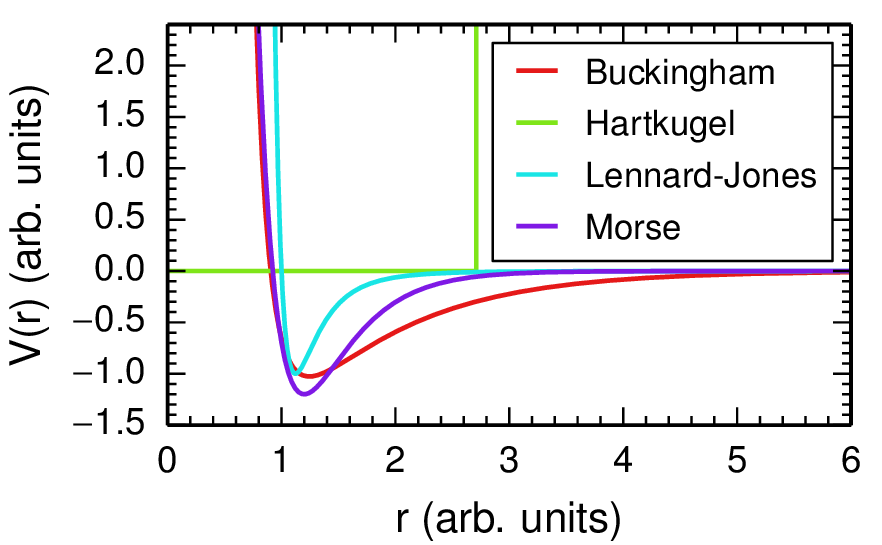
\includegraphics[width=0.5\textwidth]{mdpotplot}
  \caption{Beispiele einfacher Paarpotentiale}
  \label{fig:mdpairpotentials}
\end{figure}

Zwar zeigen Paarpotentiale gute thermodynamische Eigenschaften bei hoher Effizienz, doch können sie aufgrund ihrer Schlichtheit kein atomistischen Strukturen verlässlich vorhersagen, weshalb die umfangreicheren Mehrteilchen-Potentiale entwickelt wurden.

\subsubsection{N-Teilchen-Potentiale}

N-Teilchen-Potentiale erweitern Paarpotentiale um weitere Terme, die von einer festen Anzahl an Teilchen abhängen, beispielsweise Winkel- und Torsionsabhängigkeiten.

\begin{equation}
  \label{eq:nbody-energy}
  E = \sum_i\sum_{j \neq i}{V_2\left(r_{ij}\right)} + \sum_i\sum_{j \neq i}\sum_{i \neq k \neq j}{V_3\left(r_{ij}, r_{ik}, \theta_{ijk}\right)} + \dots
\end{equation}
\todo{letzte Summe: Indizes aufspalten}

Obwohl sich mit N-Teilchen-Potentialen komplexere Systeme betrachten lassen, zeigen sie die gleichen Schwachstellen wie Paarpotentiale, benötigen aber eine größere Anzahl an Parametern,
Zwar gibt es erfolgreiche \todo{kommerzielle} Anwendungen für Biomoleküle (\todo{CHARMM} \todo{GROMACS} \todo{AMBER}), die allerdings aufgrund ihrer Spezialisierung nicht auf andere Stoffsysteme wie Festkörper oder Oberflächen übertragbar sind.

\subsubsection{Embedded Atom Model}

Das Embedded Atom Model (EAM) besteht aus einem Paarpotential $V_{\alpha\beta}(r_{ij})$ für jedes Atom $i$ sowie einer Einbettungsfunktion $F_\alpha$, die die Energie des Atomes in Abhängigkeit der angenäherten lokalen Elektronendichte $\rho_\beta(r_{ij})$ modelliert (Gleichung \ref{eq:eam-energy}).\todo{Referenz}
So lassen sich metallische Bulks und Oberflächen simulieren, für die $\alpha$ und $\beta$ verschiedene Atomsorten darstellen, doch führt die Formulierung für andere Systeme zwangsläufig zur Bildung gleichatomiger Cluster.
Für eine Vielzahl an Metallen und Legierungen findet man in \todo{wie beispielsweise ASD}Potentialdatenbanken fertige Parametrisierungen\todo{Referenz auf Datenbank und passende Paper}, von denen viele zusätzlich zu den strukturellen Eigenschaften auch thermodynamisches Verhalten recht gut modellieren (Abschnitt \ref{goldthermo}).

\begin{equation}
  \label{eq:eam-energy}
  E = \sum_i\left[F_\alpha\left(\sum_{j\neq i}{\rho_\beta\left(r_{ij}\right)}\right) + \frac{1}{2}\sum_{j\neq i}{V_{\alpha\beta}\left(r_{ij}\right)}\right]
\end{equation}

\subsubsection{Modified Embedded Atom Model}

Als Erweiterung des EAM-Potentials wurden MEAM-Potentiale entwickelt, die neben Metallen und Legierungen auch Metalloxide und andere Mischsysteme ermöglichen sollen. \todo{Referenz auf Baskes}
Sie basieren auf dem gleichen Grundgedanken, stellen die Einbettungsenergie aber in Abhängigkeit einer umfangreicheren Formulierung der lokalen Elektronendichte dar.
An dieser Stelle soll neben der oberflächlichen Formel in Gleichung \ref{eq:meam-energy} auf die ursprüngliche Publikation von Baskes \todo[inline]{Ref!} verwiesen werden.

\begin{equation}
  \label{eq:meam-energy}
  E = \sum_i\left[F_\alpha\left(\bar{\rho_i}\right) + \frac{1}{2}\sum_{j\neq i}{V_{ij}\left(r_{ij}\right)}\right]
\end{equation}

\subsubsection{Reactive Force Fields}

\todo{Referenz auf van Duin}
todo[inline]{continuehere}
Reactive Force Fields (ReaxFF) wurden mit der Idee entwickelt, bisher unmögliche Simulationen in Molekulardynamik mit größeren Systemen darstellen zu können.
Dafür fließt eine Vielzahl an Einflüssen in die Potentialparameter ein, beispielsweise Van-der-Waals-Kräfte und elektrostatische Kräfte, allerdings ist der zentrale Gedanke die Modellierung von Über- und Unterkoordination eines Atomes in seiner Nachbarschaft unter Ladungsaustausch.
Somit lassen sich Bindungen während der Simulation dynamisch formen und lösen und dadurch ganze Reaktionen zwischen verschiedenen Molekülen simulieren.

\begin{align}
  \label{eq:reax-formulation}
  E_\text{system} &= E_\text{bond} + E_\text{lp} + E_\text{over} + E_\text{under} + E_\text{val} + E_\text{pen} + E_\text{coa} + E_\text{C2} \\
  \nonumber  & + E_\text{tors} + E_\text{conj} + E_\text{H-bond} + E_\text{vdWaals} + E_\text{Coulomb}
\end{align}

Die meisten Terme der Gesamtenergie werden über die Bindungsordnung berechnet, die über Beiträge für $\sigma$-, $\pi$- und Doppel-$\pi$-Bindungen aus dem Bindungsabstand errechnet wird.
Einige werden durch Taper-Korrektur\todo{ref} in der Nähe des Cutoff-Abstands auf 0 gesenkt, um Diskontinuitäten zu vermeiden und einen fließenden Übergang zwischen Bindungszuständen zu ermöglichen.

\todo{Referenz auf Equations\_Reax.pdf}

\begin{table}
  \begin{tabularx}{\textwidth}{|llX|}
    \hline
    \textbf{Term}      & \textbf{Beitrag}            & \textbf{Kommentar}                            \\
    \hline
    $E_\text{bond}$    & Bindungsenergien            & Berechnung über Bindungsordnung               \\
    $E_\text{lp}$      & freie Elektronenpaare       & über Bindungsordnungssumme am Atomzentrum     \\
    $E_\text{over}$    & Überkoordinationen          & unter Ausschluss freier Elektronenpaare       \\
    $E_\text{under}$   & Unterkoordinationen         & nur bei unterkoordinierten $\pi$-Bindungen    \\
    $E_\text{val}$     & Bindungswinkel              & Optimum abhängig von Elektronenkonfiguration  \\
    $E_\text{pen}$     & Strafenergien               & Fehlerkorrektur bei Winkeln mit Doppelbindung \\
    $E_\text{coa}$     & Drei-Teilchen-Konjugationen & Stabilisierung von NO$_2$-Gruppen             \\
    $E_\text{C2}$      & Dreifachbindungskorrektur   & Stabilisierung der Dreifachbindung von C$_2$  \\
    $E_\text{tors}$    & Torsionsbarrieren           &                                               \\
    $E_\text{conj}$    & Vier-Teilchen-Konjugationen & Konjugation bei Kohlenwasserstoffen           \\
    $E_\text{H-bond}$  & Wasserstoffbrücken          &                                               \\
    $E_\text{vdWaals}$ & Van-der-Waals-Kräfte        &                                               \\
    $E_\text{Coulomb}$ & Coulomb-Kräfte              &                                               \\
    \hline
  \end{tabularx}
  \caption[ReaxFF Energiebeiträge]{ReaxFF Energiebeiträge aus Gleichung \ref{eq:reax-formulation}}
  \label{tab:reax-energies}
\end{table}

Wie aus Gleichung \ref{eq:reax-formulation} und Tabelle \ref{tab:reax-energies} hervor geht, wurden das ReaxFF-Potential ursprünglich für Reaktionen von organischen Molekülen entwickelt, ist aber vielseitig genug, eine Vielzahl anderer Materialien simulieren zu können.
Die unterstützten Stoffgruppen hängen dabei stark von den Strukturen ab, an die die Parametrisierung gefittet wurde.
Auch, wenn alle notwendigen Atomsorten unterstützt werden, kommt es häufig vor, dass der zu untersuchende Stoff bei der Parametersuche nicht beachtet wurde und somit nicht darstellbar ist.

In den letzten fünf Jahren haben Reactive Force Fields jedoch langsam an Aufmerksamkeit gewonnen, so dass die Zahl spezialisierter Parametrisierungen wächst.
Es gibt auch Bestrebungen, sich ergänzende ReaxFF-Parametrisierungen zu kombinieren und somit mit einer Parametrisierung jedes gewünschte System betrachten zu können.
Besonders in kommerzieller MD-Software\todo{Referenz auf GULP} versucht man so, dem Nutzer unnötige Arbeit abzunehmen.
Es muss sich jedoch noch zeigen, ob dieser Ansatz zufrieden stellende Ergebnisse liefern kann.

\subsubsection{Allgemeine Probleme}

\textbf{Parametrisierung}:
Da Molekulardynamik keine ab-initio-Methode ist, sondern jedes Potential erst an experimentelle oder numerische Daten angepasst (gefittet)\todo{was nun?} werden muss, sollte die Herkunft jeder Parametrisierung bei seiner Nutzung bedacht werden.
\todo{kulkarni: Kritische Betrachtung seiner Trainingsstrukturen}
\\\\
\textbf{Übertragbarkeit}:
Je nach Potentialart lassen sich viele Parametrisierungen nicht vermischen oder auf andere Probleme übertragen.
\\\\
\textbf{Analysemethoden}:
Im Normalfall sind Potentiale entweder für strukturelle oder thermodynamische Größen optimiert.
Mit einem rein strukturellen Potential lassen sich also keine thermodynamischen Größen und Phasenübergänge verlässlich ermitteln.
\\\\
\textbf{Reaktionen}:
Mit der Ausnahme des ReaxFF-Potentiales lassen sich per Molekulardynamik keine Reaktionen betrachten.
\\\\
\textbf{Annäherungen}:
\todo{Was hast du hier gedacht, Erik?}

\subsection{Auswertung}

\subsubsection{Relaxierungen}

\subsubsection{Struktur}

Zur Auswertung einer Struktur bietet sich zuerst eine visuelle Beurteilung an, die mit entsprechenden Programmen vorgenommen werden kann.
Damit können grobe Defekte ausgeschlossen werden.

\subsubsection{Dichte}

Die Dichte lässt sich bei periodischen Strukturen nach über Volumen und

\subsubsection{Radiale Verteilungsfunktionen}

\subsubsection{Oberfläche}

Die Oberfläche einer Struktur gibt Hinweise auf angelagerte Moleküle, Rauheit, Porösität und Bildung von Cluster und Nanopartikeln.
Bei großen, glatten Strukturen reicht oft ein Schnitt entlang einer Hauptachse, um Bulk und Oberfläche zu trennen.
In den verbliebenen Fällen lässt sich zu diesem Zweck eine Alpha-Form per Delaunay-Triangulation bestimmen (Abschnitt \ref{datadelaunay}.
Die eigentlichen Untersuchungen beschränken sich dann auf eine Zählung der Bindungen und Atomsorten, Radiale Verteilungsfunktionen, Messungen der Oberfläche oder Abweichungen der Schichtdicke vom Mittelwert.

\subsubsection{Reaktionen}



\subsection{Software}

Für molekulardynamische Simulationen gibt es sowohl kommerzielle als auch freie Softwarepakete, die einige Parametersätze mitbringen.
Tabelle \ref{tab:mdsoftware} stellt eine Auswahl daraus dar.

\begin{table}
  \oddrowcolors
  \caption[MD-Software]{MD-Software}
  \label{tab:mdsoftware}
  \begin{tabularx}{\textwidth}{|llX|}
    \hline
    \textbf{Paket} & \textbf{Rechteinhaber} & \textbf{Kommentare} \\
    \hline
    LAMMPS & SANDIA & quelloffen, CLI-bedienbar, Bibliothek, eigene Potentiale möglich \\
    Materials Studio GULP & Accelrys & Tief in graphischer Oberfläche verankert \\
    AMBER & University of California & verschiedene Biomoleküle \\
    CHARMM & Accelrys & Proteine \\
    GROMACS & Uppsala University & Biomoleküle, quelloffen \\
    \hline
  \end{tabularx}
  \todo[inline]{References!}
  \todo[inline]{bessere Beschreibung!}
\end{table}

